\documentclass{../qh_exercise}
\graphicspath{ {./images/} }

\begin{document}

\section{Leerdoelen}
\begin{itemize}
    \item Ingewikkelde fractels kunnen tekenen
    \item Snappen wat een L-System is
    \item Extra: L-Systems kunnen gebruiken om fractels te tekenen
\end{itemize}

\section{Uitleg}
\begin{itemize}
    \item \myhref{https://www.youtube.com/watch?v=-wiverLQl1Q\&list=PLRqwX-V7Uu6bXUJvjnMWGU5SmjhI-OXef\&index=1}{Fractals - The Nature of Code}\\
    Alleen \textbf{8.4, 8.5, cc\#14, cc\#16}\\
    \item \myhref{https://natureofcode.com/book/chapter-8-fractals/}{Chapter 8. Fractals}\\
    Alleen \textbf{8.6}\\
\end{itemize}

\newpage
\section{Opdrachten}
Deze opdracht bestaat uit twee delen. Het eerste deel (het maken van een Sierpinski Triangle) hoort nog bij de stof. En het tweede deel over L-Systems is verdieping en hoef je niet te kunnen/kennen (hoewel het wel super gaaf is!).

\subsection{Sierpinski Triangle}
Maak een functie die een Sierpinski Triangle tekent:
\begin{lstlisting}
void sierpinski(int n, PVector p1, PVector p2, PVector p3) {
}
\end{lstlisting}
Een Sierpinski Triangle (zie figuur \ref{fig:sierpinski}) bestaat uit een driehoek met hoekpunten \texttt{p1, p2, p3}. Telkens wordt het midden van de zijden bepaald. Deze middelpunten vormen samen met de orginele hoekpunten 3 kleinere driehoeken. Dit proces wordt \texttt{n} keer recursief herhaald zodat figuur \ref{fig:sierpinski} ontstaat!

Je mag gebruik maken van de volgende functie:
\begin{lstlisting}
PVector midpoint(PVector p1, PVector p2) {
  return p1.copy().add(p2).mult(0.5);
}
\end{lstlisting}

\begin{figure}[H]
	\centering
	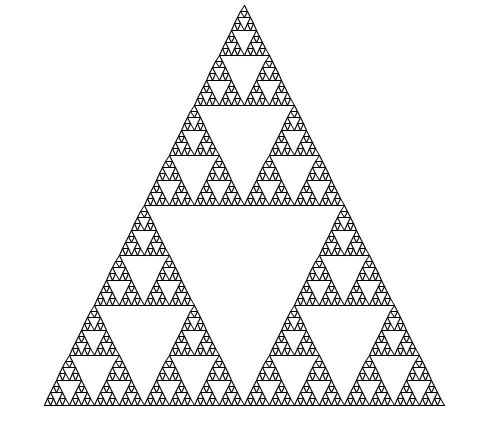
\includegraphics[width=8cm]{sierpinski.png}
	\caption{Sierpinski's Triangle met n = 5}
	\label{fig:sierpinski}
\end{figure}

\newpage
\subsection{[Extra] L-Systems}
Lees de paragraaf over L-Systems of bekijk de video's (zie het kopje uitleg). 
\subsubsection{Eerste L-System}
\begin{verbatim}
Axiom = A
Rules:
    A -> B-A-B
    B -> A+B+A
\end{verbatim}
De eerste generatie van dit L-System geeft \texttt{B-A-B}\\
De tweede generatie geeft \texttt{A+B+A-B-A-B-A+b+A}\\
Geef zelf generatie drie.

\subsubsection{Tweede L-Systems}
\begin{verbatim}
    Axiom = F-G-G
    Rules:
        F -> F-G+F+G-F
        G -> GG
\end{verbatim}
Geef generatie twee van dit L-System (is een boel schrijfwerk, maar het waard!)

\subsubsection{Turtle Graphics}
We gaan nu zogenaamde \textbf{turtle graphics} toepassen op het tweede L-System. Zet je pen op het papier en lees je antwoord van de vorige opdracht letter voor letter:
\begin{description}
    \item[Als je een F tegenkomt] zet een streep van 1 cm (omhoog).
    \item[Als je een G tegenkomt] zet een streep van 1 cm (omhoog).
    \item[Als je een + tegenkomt] draai het paoier 120 graden met de klok mee.
    \item[Als je een - tegenkomt] draai het papier 120 graden tegen de klok in.
\end{description}
Als je verder wil spelen met deze L-Systems, je kunt heel veel leuke dingen op het internet vinden. \myhref{http://www.kevs3d.co.uk/dev/lsystems/}{Deze geweldige site:}

\end{document}